%% Included in decks: slidemage-manual, slidemage-manual-copy
%%

% SlideMage manual, chapter "Accessibility": drafting image descriptions with a local
% model, and reviewing them. The strip is a crop of the Images page's model pickers
% (tools/manual/make_screenshots.py). What the page holds: slide 1ih.
\setSlideVersion{1-0-0+}
\begin{standardframe}{Drafting and reviewing descriptions}
	\small
	Describing every image by hand is slow, so, with the Ollama or Claude plugin, a
	vision model can write a first version. You then check and correct each one: a draft is only a
	starting point.
	\par\smallskip
	\centering
	{\setlength{\fboxsep}{0pt}\fcolorbox{c_primary_gray}{white}{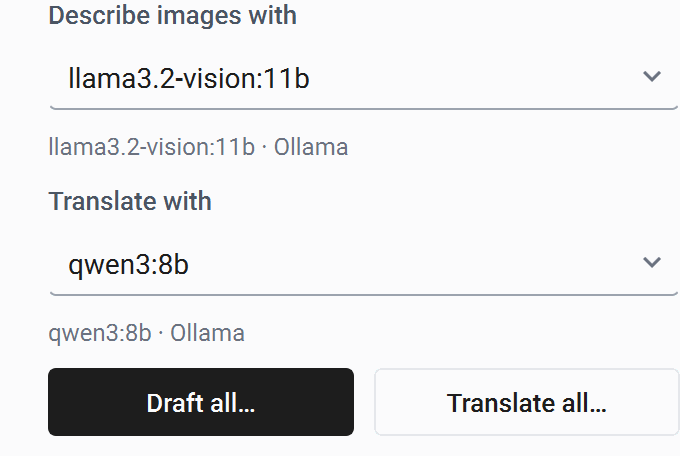
\includegraphics[width=\dimexpr0.3\linewidth-0.8pt\relax]{media/screenshot-slidemage-images-toolbar.png}}}
	\par\smallskip
	\raggedright
	\begin{columns}[T,onlytextwidth]
		\begin{column}{0.52\linewidth}
			\textbf{Drafting}
			\shrinklists{3}
			\begin{itemize}
				\item \emph{Draft this slide}: the open slide's images, with the model picked under the list
				\item \emph{Draft all\ldots}: every image without a description, unattended; each is saved as it finishes, so you can stop and go on later
				\item \emph{Tune prompt\ldots}: redo one image with an edited prompt
				\item \emph{Clear draft}: drops unreviewed drafts, never a reviewed text
			\end{itemize}
		\end{column}
		\begin{column}{0.45\linewidth}
			\textbf{Reviewing}
			\shrinklists{3}
			\begin{itemize}
				\item Check every draft against the image, which the page shows at full size; on faint charts the models invent numbers
				\item \emph{Save and mark reviewed} confirms the text and this slide's takeaway; a later edit withdraws the review
				\item \emph{Translate all\ldots} drafts the German texts
			\end{itemize}
		\end{column}
	\end{columns}
\end{standardframe}
